% Un articolo scritto con LaTeX
\documentclass[a4paper,11pt]{article}
\usepackage{graphicx}
\usepackage[T1]{fontenc} % codifica dei font in uscita
\usepackage[utf8]{inputenc} % lettere accentate da tastiera
\usepackage[italian]{babel} % lingua principale del documento
\usepackage{url}
\usepackage [a4paper, top=2.5cm, bottom=2.5cm, left=1.5cm, right=1.5cm, bindingoffset=8mm] {geometry}

% inizio documento

\usepackage{graphicx}
\begin{document}
\begin{center}
\textbf{\huge Esperienza VI} \\ \vspace{10pt}
\large Alberini Giacomo \\ Bassini Luigi \\ Michele Pedrotti\\ Trevisson Nicola 
\end{center}
\section{Scopo dell'esperienza}
Lo scopo di questa esperienza è quello di misurare la conduttanza di vari tubi con diametri e lunghezze diversi in regimi di flusso differenti.
\section{Misura della Conduttanza}

Per calcolare la conduttanza si è reso necessario l'uso di una pompa da vuoto, due pirani (con relativa strumentazione di misura ), una vlavola a spillo (già tarata in precedenza) e vari tubi con lunghezze e diametri differenti.

	
\begin{center} 
\begin{figure}[htpd]
\hspace{120pt}
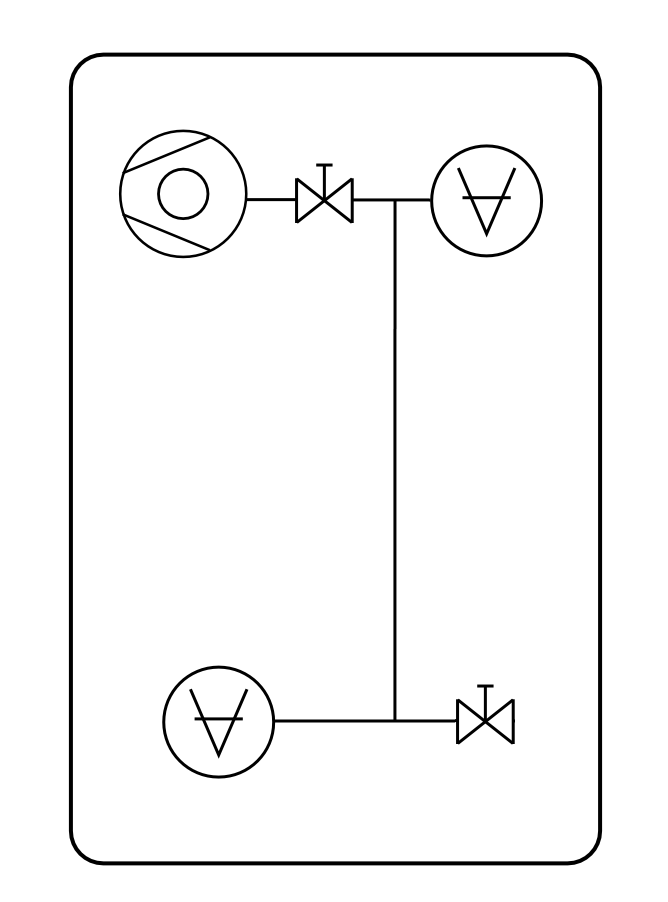
\includegraphics[scale=0.5]{schema_finale.png}
\end{figure}
\end{center}

Nello schema soprastante, per semplicità, i vari tubi sono indicati dalla linea retta verticale tra i due T che collegano i pirani.
Per ottenre il valore di conduttanza a differenti regimi di flusso, opportunamente creati tramite la manipolazione della valvola a spillo, si sono utilizzati i due pirani. Essi ci hanno permesso di rilevare i valori di pressione in testa e in coda al tubo sotto analisi. L'andamento della pressione è stato monitorato tramite un software che ha reso osservabile il momento in cui la pressione si stabilizzava dopo i cambiamenti di flusso passanti per la spillo. Una volta stabilizzata la pressione si è proceduto all'annotazione del valore di pressione corrispondente al numero di tacche di apertura della valvola a spillo (dal vuoto nel tubo per poi crescereda 4 a 8 giri e ritorno).
Una volta ottenuti tutti i dati relativi ad ogni tubo a nostra disposizione si passa al calcolo della conduttanza. Per fare questo è necessario utilizzare i dati di flusso delle precedenti esperienze relativi alla valvola a spillo. Noto il flusso Q della valvola a spillo e nota la differenza di pressione fra testa e coda $\delta p$ si può ricavare la conduttanza C tramite l'ugualianza $ C = \frac{Q}{\Delta P} $.\\
 

\begin{center} 
\begin{tabular}{|c|c|c|c|}
\hline Apertura valvola a spillo & Conduttanza & Regime di flusso & Conduttanza teorica \\ 
\hline 4 & 0.0015 $\cdot10^{-4}$ &  & 0.0046$\cdot10^{-3}$ \\ 
\hline 5 & 0.0010$\cdot10^{-4}$ &  & 0.0055$\cdot10^{-3}$ \\ 
\hline 6 & 0.0600$\cdot10^{-4}$ &  & 0.0119$\cdot10^{-3}$ \\
\hline 7 & 0.2411$\cdot10^{-4}$ &  & 0.0457$\cdot10^{-3}$ \\
\hline 8 & 0.6802$\cdot10^{-4}$ &  & 0.1091$\cdot10^{-3}$ \\ 
\hline 
\end{tabular}\\
\vspace{5pt}
Tubo di lunghezza $8m$ e diametro $4mm$ .
\\
\vspace{15pt}
\begin{tabular}{|c|c|c|c|}
\hline Apertura valvola a spillo & Conduttanza & Regime di flusso & Conduttanza teorica \\ 
\hline 4 & 0.0005$\cdot10^{-3}$ &  & 0.0070$\cdot10^{-3}$ \\ 
\hline 5 & 0.0010$\cdot10^{-3}$ &  & 0.0086$\cdot10^{-3}$ \\ 
\hline 6 & 0.0231$\cdot10^{-3}$ &  & 0.0329$\cdot10^{-3}$ \\
\hline 7 & 0.0957$\cdot10^{-3}$ &  & 0.1393$\cdot10^{-3}$ \\
\hline 8 & 0.2461$\cdot10^{-3}$ &  & 0.4015$\cdot10^{-3}$ \\ 
\hline 
\end{tabular}\\
\vspace{5pt}
Tubo di lunghezza $80cm$ e diametro $4mm$.
\\
\vspace{15pt}
\begin{tabular}{|c|c|c|c|}
\hline Apertura valvola a spillo & Conduttanza & Regime di flusso & Conduttanza teorica \\ 
\hline 4 & 0.0070$\cdot10^{-4}$ &  & 0.0014$\cdot10^{-3}$ \\ 
\hline 5 & 0.0027$\cdot10^{-4}$ &  & 0.0026$\cdot10^{-3}$ \\ 
\hline 6 & 0.0952$\cdot10^{-4}$ &  & 0.0114$\cdot10^{-3}$\\
\hline 7 & 0.3585$\cdot10^{-4}$ &  & 0.0496$\cdot10^{-3}$ \\
\hline 8 & 0.9404$\cdot10^{-4}$ &  & 0.1262$\cdot10^{-3}$ \\ 
\hline 
\end{tabular}\\
\vspace{5pt}
Tubo di lunghezza $80cm$ e diametro $2.5mm$.
\\
\vspace{15pt}
\begin{tabular}{|c|c|c|c|}
\hline Apertura valvola a spillo & Conduttanza & Regime di flusso & Conduttanza teorica \\ 
\hline 4 & 0.0005$\cdot10^{-4}$ &  & 0.0126$\cdot10^{-3}$ \\ 
\hline 5 & 0.0008$\cdot10^{-4}$ &  & 0.0149$\cdot10^{-3}$ \\ 
\hline 6 & 0.0248$\cdot10^{-4}$ &  & 0.0428$\cdot10^{-3}$ \\
\hline 7 & 0.1046$\cdot10^{-4}$ &  & 0.1537$\cdot10^{-3}$ \\
\hline 8 & 0.1087$\cdot10^{-4}$ &  & 0.9663$\cdot10^{-3}$ \\ 
\hline 
\end{tabular}\\
\vspace{5pt}
Tubo di lunghezza $8m$ e diametro $2.5mm$.
\\
\vspace{15pt}
\begin{tabular}{|c|c|c|c|}
\hline Apertura valvola a spillo & Conduttanza & Regime di flusso & Conduttanza teorica \\ 
\hline 4 &  &  &  \\ 
\hline 5 &  &  &  \\ 
\hline 6 &  &  &  \\
\hline 7 &  &  &  \\
\hline 8 &  &  &  \\ 
\hline 
\end{tabular}\\
Composizione di due tubi di acciaio in serie con tre vacuometri in tre punti dell'impianto, uno in testa, uno in coda e uno in posizione intermedia fra i due tubi.
\vspace{10pt}
\end{center}



\end{document}